\chapter{Requirement Analysis}
\label{chap:requirement-analysis}

\section{Stakeholder Analysis}
\label{section:stakeholder-analysis}

The following stakeholders have been identified for the system:

\begin{enumerate}
    \item \textbf{Investigators.} Security personnel, law enforcement officers, and loss prevention staff who actively search footage for specific people, objects, or events. Their primary concern is retrieval accuracy and the ability to use natural language, reference images, and face recognition to locate evidence quickly.

    \item \textbf{Facility Operators.} Business owners, operations managers, and other non-technical users who review footage to verify incidents, check deliveries, or monitor daily operations. Their primary concern is ease of use — the system must be operable without technical expertise.

    \item \textbf{System Administrator.} Technical staff responsible for deploying and maintaining the system, managing video storage, and ensuring the processing pipeline runs reliably.
\end{enumerate}

Both Investigators and Facility Operators have access to all features (upload, search, face recognition, export). They differ in their priorities, not their permissions.

\section{User Stories and Use Cases}
\label{section:user-stories-use-cases}

\subsection{User Stories}

\begin{enumerate}
    \item As a \textbf{user}, I want to upload video files and have them automatically processed and indexed so that the footage becomes searchable without manual intervention.
    \item As a \textbf{user}, I want to search footage by describing a person or object in natural language so that I can quickly locate relevant moments without manually reviewing hours of video.
    \item As a \textbf{user}, I want to upload a reference photo and find all matching appearances so that I can track a person or object across cameras.
    \item As a \textbf{user}, I want to select a detected face and see every frame where that individual appears so that I can build a timeline of their activity.
    \item As a \textbf{user}, I want to click on a search result and jump directly to that moment in the video so that I can review the context around the event.
    \item As a \textbf{user}, I want to export selected search results with timestamps and metadata so that I can compile evidence or share findings.
\end{enumerate}

\subsection{Use Cases}

\begin{table}[H]
\centering
\begin{tabular}{|l|p{10cm}|}
\hline
\textbf{Use Case}       & UC-1: Text-Based Video Search \\ \hline
\textbf{Primary Actor}   & User \\ \hline
\textbf{Preconditions}   & Video footage has been uploaded and processed. The segmentation and encoding pipeline has completed, and region embeddings are stored in the vector database. \\ \hline
\textbf{Postconditions}  & The user receives a ranked list of video moments matching their query, each linked to the corresponding timestamp. \\ \hline
\textbf{Main Success Scenario} &
    \begin{enumerate}[nosep, leftmargin=*]
        \item The user navigates to the search interface.
        \item The user enters a natural language query (e.g., ``person carrying a cardboard box'').
        \item The system encodes the query text using SigLIP2 \cite{zhai2025siglip2}.
        \item The system performs cosine similarity search against stored region embeddings.
        \item The system returns a ranked list of matching results with thumbnail previews and timestamps.
        \item The user clicks on a result to jump to that moment in the video player.
    \end{enumerate} \\ \hline
\textbf{Alternative Flows} &
    \begin{itemize}[nosep, leftmargin=*]
        \item \textit{No results found:} The system displays a message indicating no matches and suggests broadening the query.
        \item \textit{Low-confidence results:} The system returns results but flags them with lower similarity scores.
    \end{itemize} \\ \hline
\end{tabular}
\caption{UC-1: Text-Based Video Search}
\label{tab:uc1}
\end{table}

\begin{table}[H]
\centering
\begin{tabular}{|l|p{10cm}|}
\hline
\textbf{Use Case}       & UC-2: Image-Based Video Search \\ \hline
\textbf{Primary Actor}   & User \\ \hline
\textbf{Preconditions}   & Video footage has been uploaded and processed. Region embeddings are stored in the vector database. \\ \hline
\textbf{Postconditions}  & The user receives a ranked list of visually similar regions with timestamps. \\ \hline
\textbf{Main Success Scenario} &
    \begin{enumerate}[nosep, leftmargin=*]
        \item The user navigates to the search interface.
        \item The user uploads a reference image (e.g., a photo of a suspect or a specific item).
        \item The system encodes the uploaded image using SigLIP2's image encoder \cite{zhai2025siglip2}.
        \item The system performs cosine similarity search against stored region embeddings.
        \item The system returns a ranked list of matching results with thumbnails, similarity scores, and timestamps.
        \item The user clicks on a result to jump to that moment in the video player.
    \end{enumerate} \\ \hline
\textbf{Alternative Flows} &
    \begin{itemize}[nosep, leftmargin=*]
        \item \textit{Invalid file format:} The system rejects the upload and prompts the user to provide a supported image format (JPEG, PNG, WebP).
        \item \textit{No results found:} The system displays a message indicating no visual matches were found.
    \end{itemize} \\ \hline
\end{tabular}
\caption{UC-2: Image-Based Video Search}
\label{tab:uc2}
\end{table}

\begin{table}[H]
\centering
\begin{tabular}{|l|p{10cm}|}
\hline
\textbf{Use Case}       & UC-3: Face Search \\ \hline
\textbf{Primary Actor}   & User \\ \hline
\textbf{Preconditions}   & Video footage has been uploaded and processed. Face detection and clustering have completed. \\ \hline
\textbf{Postconditions}  & The user receives a chronological list of all frames containing the selected individual. \\ \hline
\textbf{Main Success Scenario} &
    \begin{enumerate}[nosep, leftmargin=*]
        \item The user navigates to the face gallery page.
        \item The system displays all detected face clusters, each shown as a representative thumbnail with the number of appearances.
        \item The user selects a face cluster.
        \item The system retrieves all frames where that individual was detected using InsightFace embeddings.
        \item The system displays results in chronological order with timestamps and source camera labels.
        \item The user clicks on a result to view the footage at that moment.
    \end{enumerate} \\ \hline
\textbf{Alternative Flows} &
    \begin{itemize}[nosep, leftmargin=*]
        \item \textit{No faces detected:} The footage contains no detectable faces (e.g., low resolution, no people present). The face gallery is empty.
    \end{itemize} \\ \hline
\end{tabular}
\caption{UC-3: Face Search}
\label{tab:uc3}
\end{table}

\begin{table}[H]
\centering
\begin{tabular}{|l|p{10cm}|}
\hline
\textbf{Use Case}       & UC-4: Video Upload and Processing \\ \hline
\textbf{Primary Actor}   & User \\ \hline
\textbf{Preconditions}   & The system is running and the user is authenticated. \\ \hline
\textbf{Postconditions}  & The uploaded footage is fully indexed and searchable. \\ \hline
\textbf{Main Success Scenario} &
    \begin{enumerate}[nosep, leftmargin=*]
        \item The user navigates to the upload page.
        \item The user selects one or more video files to upload.
        \item The system validates the file format and begins uploading.
        \item Once the upload completes, the system queues an asynchronous background job for processing. The user is free to navigate away or continue using the application.
        \item The background job extracts keyframes at 1--5 FPS, runs SAM segmentation \cite{kirillov2023segment}, SigLIP2 encoding \cite{zhai2025siglip2}, temporal aggregation (TAM, see Section~\ref{subsubsec:tam}), and InsightFace face detection \cite{deng2019arcface} on each frame.
        \item The system displays a progress indicator showing the current stage and percentage complete.
        \item Once processing finishes, the system marks the video as searchable and notifies the user.
    \end{enumerate} \\ \hline
\textbf{Alternative Flows} &
    \begin{itemize}[nosep, leftmargin=*]
        \item \textit{Unsupported format:} The system rejects the file and displays a list of supported formats (MP4, AVI, MOV, MKV).
        \item \textit{Processing failure:} The pipeline encounters a corrupted frame or runs out of memory. The system logs the error, skips the problematic frame, and continues processing the remaining frames.
        \item \textit{User cancellation:} The user cancels the processing job. The system stops the pipeline and discards partially processed data.
    \end{itemize} \\ \hline
\end{tabular}
\caption{UC-4: Video Upload and Processing}
\label{tab:uc4}
\end{table}

\begin{table}[H]
\centering
\begin{tabular}{|l|p{10cm}|}
\hline
\textbf{Use Case}       & UC-5: Multi-Camera Cross Search \\ \hline
\textbf{Primary Actor}   & User \\ \hline
\textbf{Preconditions}   & Footage from multiple cameras has been uploaded, processed, and indexed. \\ \hline
\textbf{Postconditions}  & The user receives a unified, ranked list of results spanning all cameras with source camera labels and timestamps. \\ \hline
\textbf{Main Success Scenario} &
    \begin{enumerate}[nosep, leftmargin=*]
        \item The user navigates to the search interface.
        \item The user enters a text query or uploads a reference image.
        \item The system encodes the query and performs similarity search across all indexed cameras.
        \item The system returns a ranked list of results from all cameras, each labeled with the source camera and timestamp.
        \item The user clicks on a result to jump to that moment in the corresponding camera's footage.
    \end{enumerate} \\ \hline
\textbf{Alternative Flows} &
    \begin{itemize}[nosep, leftmargin=*]
        \item \textit{Single camera indexed:} The system behaves identically to UC-1 or UC-2.
    \end{itemize} \\ \hline
\end{tabular}
\caption{UC-5: Multi-Camera Cross Search}
\label{tab:uc5}
\end{table}

\begin{table}[H]
\centering
\begin{tabular}{|l|p{10cm}|}
\hline
\textbf{Use Case}       & UC-6: Time-Filtered Search \\ \hline
\textbf{Primary Actor}   & User \\ \hline
\textbf{Preconditions}   & Video footage has been uploaded and processed. The footage contains valid timestamp metadata. \\ \hline
\textbf{Postconditions}  & The user receives search results limited to the specified time range. \\ \hline
\textbf{Main Success Scenario} &
    \begin{enumerate}[nosep, leftmargin=*]
        \item The user navigates to the search interface.
        \item The user sets a date and time range filter.
        \item The user enters a text query, uploads a reference image, or selects a face cluster.
        \item The system restricts the search to frames within the specified time window.
        \item The system returns ranked results filtered to the selected time range.
    \end{enumerate} \\ \hline
\textbf{Alternative Flows} &
    \begin{itemize}[nosep, leftmargin=*]
        \item \textit{No results in range:} The system displays a message suggesting the user broaden the time window.
    \end{itemize} \\ \hline
\end{tabular}
\caption{UC-6: Time-Filtered Search}
\label{tab:uc6}
\end{table}

\begin{table}[H]
\centering
\begin{tabular}{|l|p{10cm}|}
\hline
\textbf{Use Case}       & UC-7: Export Search Results \\ \hline
\textbf{Primary Actor}   & User \\ \hline
\textbf{Preconditions}   & A search has been performed and results are displayed. \\ \hline
\textbf{Postconditions}  & The user downloads a file containing the selected results with associated metadata. \\ \hline
\textbf{Main Success Scenario} &
    \begin{enumerate}[nosep, leftmargin=*]
        \item The user performs a search and reviews the results.
        \item The user selects one or more results to export.
        \item The system generates downloadable files containing the matched frames as screenshots or short video clips, along with metadata (timestamp, source camera, similarity score).
        \item The user downloads the exported file.
    \end{enumerate} \\ \hline
\textbf{Alternative Flows} &
    \begin{itemize}[nosep, leftmargin=*]
        \item \textit{No results selected:} The export button is disabled until the user selects at least one result.
    \end{itemize} \\ \hline
\end{tabular}
\caption{UC-7: Export Search Results}
\label{tab:uc7}
\end{table}

\section{Use Case Diagrams}
\label{section:use-case-diagrams}

\begin{figure}[H]
    \centering
    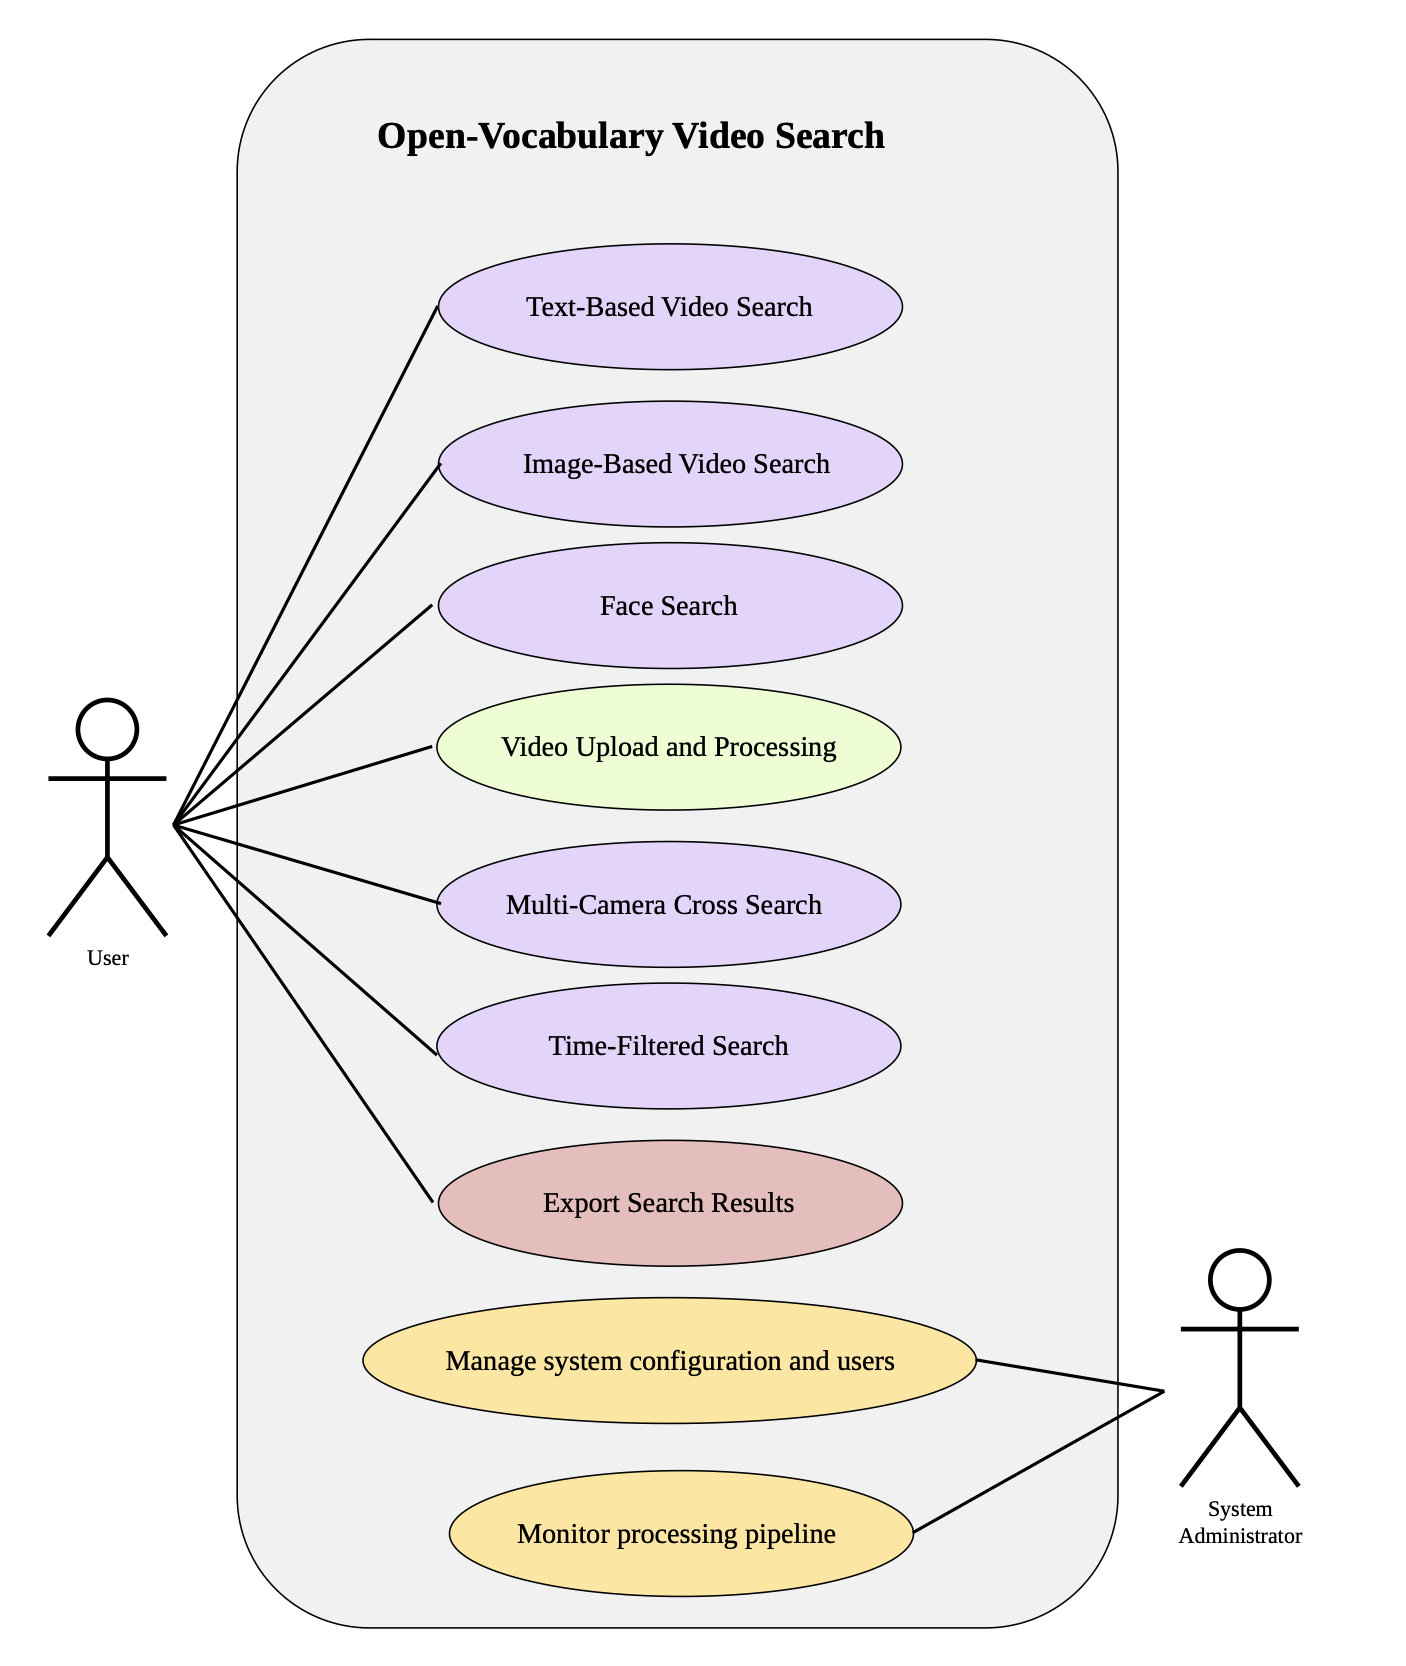
\includegraphics[width=0.8\textwidth]{assets/use-case.png}
    \caption{Use case diagram.}
    \label{fig:use-case}
\end{figure}

The system involves two actors: the \textbf{User} and the \textbf{System Administrator}. The User has access to all core functionality including uploading footage and all search modes. The System Administrator handles deployment, storage, and pipeline monitoring. The main use cases are:

\begin{itemize}
    \item UC-1: Text-based video search (User)
    \item UC-2: Image-based video search (User)
    \item UC-3: Face search (User)
    \item UC-4: Video upload and processing (User)
    \item UC-5: Multi-camera cross search (User)
    \item UC-6: Time-filtered search (User)
    \item UC-7: Export search results (User)
    \item Manage system configuration and users (System Administrator)
    \item Monitor processing pipeline (System Administrator)
\end{itemize}

\section{User Interface Design}
\label{section:user-interface-design}

\imgplaceholder{0.8\textwidth}{5cm}{UI Mockups}

The interface is organized around three main views:

\begin{enumerate}
    \item \textbf{Search View.} The primary interface where users enter text queries or upload reference images. Results are displayed as a grid of thumbnails with similarity scores and timestamps. Each result is clickable and links to the video player at the corresponding moment.

    \item \textbf{Face Gallery View.} A grid of face clusters detected across all uploaded footage. Each cluster shows a representative face thumbnail and the number of appearances. Clicking a cluster opens a chronological timeline of all frames containing that individual.

    \item \textbf{Video Player View.} An embedded video player with standard playback controls. When accessed from a search result, the player automatically seeks to the relevant timestamp. A timeline strip below the player highlights all moments that matched the current query.
\end{enumerate}
